\documentclass[a4paper]{article}
\usepackage[utf8]{inputenc}
\usepackage[T1]{fontenc}
\usepackage{graphicx}
\usepackage{hyperref}

\begin{document}

\noindent \textbf{Title}

\medskip

\noindent Nilearn: Machine learning and statistics for fMRI in Python

\bigskip

\noindent \textbf{Authors}

\medskip

\noindent Nicolas Gensollen,  Thomas Bazeille, Kshitij Chawla, Jerome-Alexis Chevalier, Kamalaker Dadi, Jérôme Dockès, Elizabeth DuPre, Daniel Gomez, Chris Gorgolewski, Alexandre Gramfort, Julia M Huntenburg, Eric Larson, Robert Luke, Chris Markiewicz, Binh Nguyen, Ana Luísa Pinho, Sylvain Takerkart, Bertrand Thirion, Alexis Thual, Taylor Tsalo, Gaël Varoquaux, Hao-Ting Wang

\bigskip

\noindent \textbf{Introduction}

\medskip

\noindent Efficient and reproducible science depends on a strong software ecosystem \cite{Poldrack2019}. We present here Nilearn, a Python package empowering the neuroimaging community by enabling fast and easy statistical learning on fMRI data: \url{https://nilearn.github.io}. It has been under continuous development for close to 10 years and is about to reach its 0.9 release. It is now part of the neuroimaging tools ecosystem with approximately 800 stars, 450 forks, and 155 contributors on GitHub, as well as more than 300 discussions on the forum \href{https://neurostars.org/}{Neurostars}.

\medskip

\noindent Nilearn provides efficient and reliable implementations of machine learning methods tailored to the needs of the neuroimaging community. It builds upon a Python "data science ecosystem" of packages such as numpy \cite{VanDerWalt2011}, scipy \cite{Oliphant2007}, scikit-learn \cite{Pedregosa2011}, and pandas \cite{McKinney2010}, that are extensively used, tested and optimized by a large scientific and industrial community. This makes it easy to use for a broad spectrum of researchers who are familiar with the Python ecosystem. Specifically, Nilearn provides methods  for decoding functional connectivity analysis, and statistical parametric mapping. It also includes datasets for teaching, and interactive visualization of brain images and connectomes.

\bigskip

\noindent \textbf{Methods}

\medskip

\noindent Nilearn is a community-led open-source project, developed and used by researchers in neuroimaging and machine-learning. It strives to be easy to use with simple code and focuses only on reliable and well-established methods. \href{https://nilearn.github.io/stable/user_guide.html}{User guides} provide an introduction to machine learning and statistics for fMRI with \href{https://nilearn.github.io/stable/auto_examples/index.html}{examples} showcasing all functionalities. Tutorials, coding sprints, as well as weekly office hours are also organized to engage the neuroimaging community.

\medskip

\noindent Nilearn uses industry-standard methods for software development: source code is version controlled, functions are covered by unit tests that are run in a Continuous Integration framework, and several reviewers check every contribution. These best practices allow to incorporate contributions from around the world while preserving the quality and reliability of the code.

\bigskip

\noindent \textbf{Results}

\medskip

\noindent Nilearn is widely used and covers many of the analysis needs for neuroimaging:

\begin{itemize}
	\item Manipulation of brain images and basic signal processing;
	\item Supervised learning and decoding;
	\item Functional connectivity and decomposition methods;
	\item Plotting;
	\item Projection of volumetric data to surfaces;
	\item General Linear Model-based analysis and statistical testing;
	\item Model selection and validation, parallelism, and caching.
\end{itemize}

\noindent In recent releases, efforts have been made on improving the visualization capabilities of Nilearn. For example, it is now possible to visualize statistical maps on the surface interactively (see fig. \ref{fig:figure_1}). In addition, most classic plotting functions can now use a "mosaic" display mode enabling to visualize cuts of the brain organized on a 2D grid.

\medskip

\noindent Nilearn also aims at making interpretation of results easier. To this end, Nilearn provides HTML reports with most of its estimators and models. Recently, reporting capabilities were added to the \textit{NiftiLabelsMasker} and the \textit{NiftiMapsMasker}, two central estimators of classical machine learning pipelines in Nilearn. Figure \ref{fig:figure_2} shows a screenshot of a \textit{NiftiMapsMasker} report, which enables browsing through spatial maps overlaid on top of a functional image.

\medskip

\noindent Nilearn is a community-driven project with an international pool of users and contributors continuously improving the tool. In order to help new contributors and organize the decision making process, the \href{https://nilearn.github.io/dev/development.html}{contributing documentations} has been largely improved.


\bigskip

\noindent \textbf{Conclusion}

\medskip

\noindent By following industry-standard methods and making analysis pipelines documented, version controlled, peer-reviewed, and shared, Nilearn targets the reproducibility crisis of neuroimaging by enabling researchers to produce pipelines that are intelligible, reproducible, and that can be extended to novel datasets.

\newpage


\begin{figure}[htp]
	\centering
	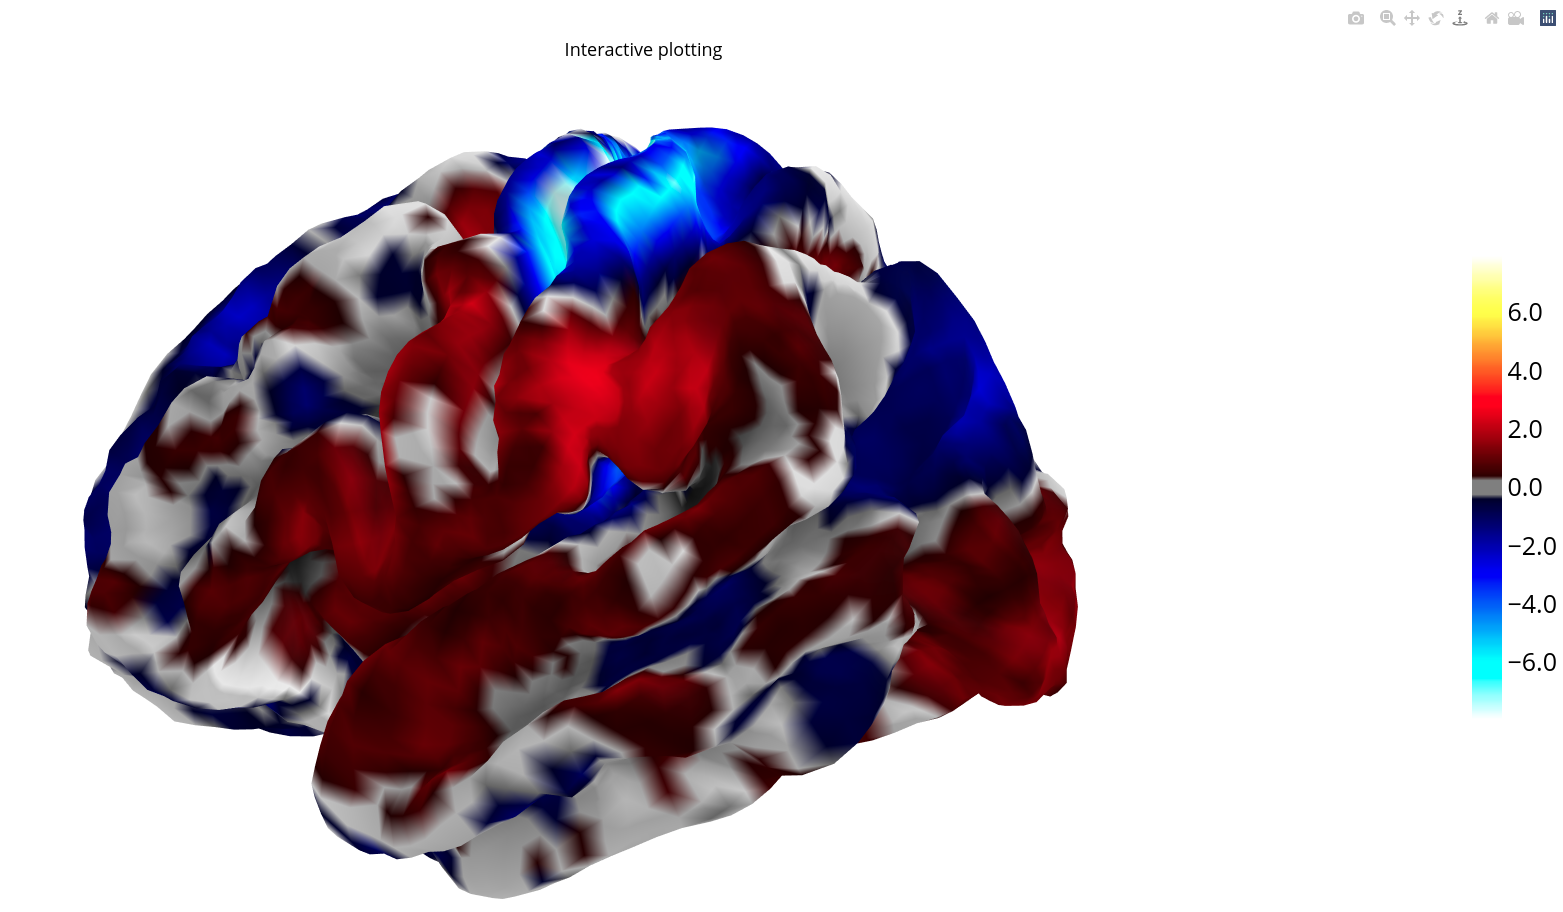
\includegraphics[scale=.25]{./figure_1}
	\caption{Example of interactively plotting a statistical map on the surface. It is possible to rotate the surface, zoom in and out...}
	\label{fig:figure_1}
\end{figure}

\begin{figure}[hbp]
	\centering
	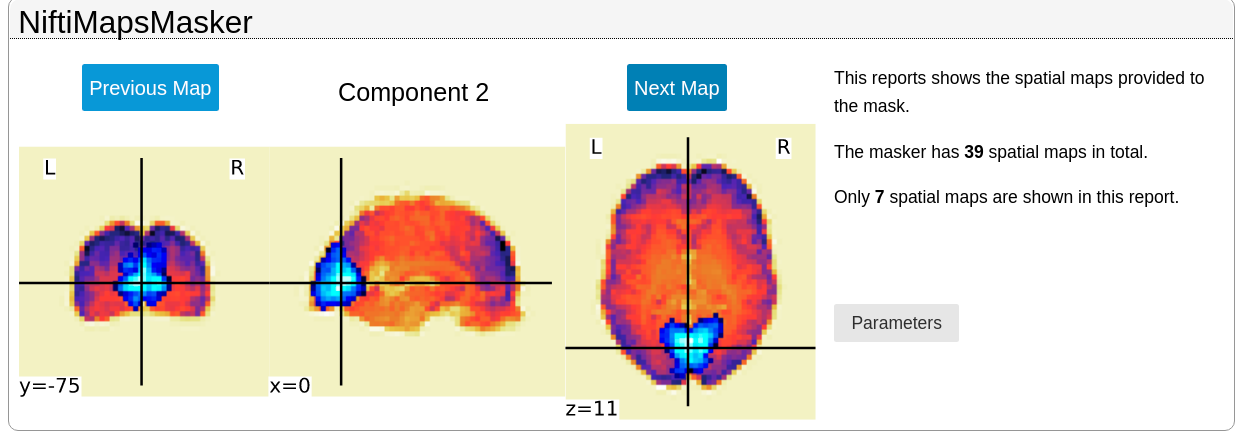
\includegraphics[scale=.33]{./figure_2}
	\caption{Example of report obtained with the NiftiMapsMasker object.}
	\label{fig:figure_2}
\end{figure}

\newpage

\bibliographystyle{plain} 
\bibliography{bibliography}

\end{document}